\chapter{强化学习在行人控制系统中的应用}

\section{环境配置}

在本研究中,我的目标是使用强化学习算法(包括\textbf{PPO}、\textbf{PID}和\textbf{DQN})对行人控制系统进行训练,并评估其在动态环境中的表现。为了实现这一目标,所有的深度学习训练和实验均在Carla仿真平台上进行。Carla平台提供了丰富的城市环境,其中包含了多种道路、建筑、车辆和行人等元素,非常适合用作自动驾驶和智能体训练的测试平台。

\textbf{Carla(Car Learning to Act)}是一个开源的自动驾驶模拟平台,专为自动驾驶研究设计。它支持多种传感器(如相机、激光雷达、IMU等)的集成,并能够模拟复杂的城市环境,包括道路、交通信号灯、行人和其他交通参与者。Carla平台为强化学习、路径规划、感知与控制算法的开发提供了一个高度可定制的虚拟环境。通过使用Carla提供的 \textbf{Python API} 来与仿真环境进行交互,控制行人的运动,并收集环境数据进行学习。该API允许我们通过编程的方式模拟行人、车辆、交通灯等各种动态因素,并能够实时获取各种传感器数据。

为了进行训练和测试以及本人电脑的算力有限,本研究选择了Carla仿真平台中的 \textbf{Town01} 地图。该地图是Carla平台提供的标准城市地图之一,包含了多种城市道路结构、交通标志、建筑物、行人以及交通工具等。具体来说:

\begin{itemize}
    \item \textbf{道路结构}:Town01包括了多条城市道路和交叉口,具有一定的复杂性,能够模拟真实城市环境中的交通流。
    \item \textbf{交通元素}:该地图还包括了不同种类的交通工具(如汽车、公交车等),以及行人和交通信号灯等。
    \item \textbf{动态障碍物}:在训练过程中,除了静态的道路和建筑外,地图中的车辆和行人会不断地动态变化,从而为智能体提供避障和路径规划的挑战。
\end{itemize}

\section{PID(Proportional-Integral-Derivative)控制算法}

\subsection{PID控制算法建模}

\subsubsection{控制方程推导}
离散PID控制算法表示为:
\begin{equation}
	u(k) = K_p e(k) + K_i T \sum_{i=0}^k e(i) + K_d \frac{e(k)-e(k-1)}{T}
\end{equation}
其中,$T=0.005s$为采样周期,$e(k)$为第$k$时刻的横向偏差。

\subsubsection{参数整定策略}
通过Ziegler-Nichols临界比例法确定基础参数后,结合实际场景进行优化:
\begin{itemize}
	\item 转向控制参数:$K_p=0.8$, $K_i=0.001$, $K_d=0.2$
	\item 速度控制参数:$K_p=0.5$, $K_i=0.01$, $K_d=0.1$
\end{itemize}

\begin{algorithm}[H]
	\caption{自适应PID控制算法}
	\begin{algorithmic}[1]
	\STATE 初始化参数$K_p^0$, $K_i^0$, $K_d^0$  % 改为 \STATE
	\WHILE{系统运行}
 	\STATE 获取激光雷达数据$L_t$
  	\STATE 计算障碍物距离$d_{obs} = \min(L_t)$
  	\IF{$d_{obs} < 5m$}
    	\STATE $K_p \gets 1.2K_p^0$
    	\STATE $K_d \gets 1.5K_d^0$
  	\ENDIF
  	\STATE 执行PID计算
	\ENDWHILE
	\end{algorithmic}
\end{algorithm}

\subsubsection{PID控制原理}
	\textbf{PID控制算法}通过以下三个分量的组合实现控制:
		\[
		u(t) = K_p e(t) + K_i \int_0^t e(\tau) d\tau + K_d \frac{d}{dt} e(t)
		\]
其中:
\begin{itemize}
    \item \textbf{比例项(P)}:$K_p e(t)$,快速响应当前误差,主导动态响应
    \item \textbf{积分项(I)}:$K_i \int e(\tau)d\tau$,消除稳态误差,补偿长期偏差
    \item \textbf{微分项(D)}:$K_d \frac{de}{dt}$,预测误差变化趋势,抑制系统震荡
\end{itemize}

\subsection{算法实现与效果可视化}

\subsubsection{传感器数据处理}
激光雷达数据处理流程包括:
\begin{enumerate}
	\item 点云预处理:滤除超出$8m$范围及非前向$60^\circ$区域的数据
	\item 障碍物聚类:采用改进DBSCAN算法,设置$\epsilon=0.5m$, $MinPts=5$
	\item 威胁评估:计算最近障碍物距离$d_{min}$及相对速度$v_{rel}$
\end{enumerate}

\subsubsection{动态权重融合算法}
目标向量$\vec{T}$与避障向量$\vec{A}$的融合策略:
\begin{equation}
	\vec{C} = \alpha \vec{T} + (1-\alpha)\vec{A}
\end{equation}
其中权重系数$\alpha$的动态调整规则为:
\begin{equation}
    \alpha = 
    \begin{cases}
        0.05, & d_{\text{min}} \leq 1\ \text{m} \\
        0.8(1 - e^{-0.5d_{\text{min}}}), & 1\ \text{m} < d_{\text{min}} \leq 5\ \text{m} \\
        1, & d_{\text{min}} > 5\ \text{m}
    \end{cases}
\end{equation}

\subsubsection{核心模块功能解析}
\begin{itemize}
    \item \textbf{PIDController类}:
    \begin{itemize}
        \item \texttt{compute()}:实现带抗饱和的PID计算
        \item \texttt{reset()}:碰撞后积分清零,防止历史误差累积
    \end{itemize}
    
    \item \textbf{PIDPedestrianEnv类}:
    \begin{itemize}
        \item \texttt{\_process\_lidar()}:实时处理激光雷达点云
        \begin{itemize}
            \item 前向60°扇形区域检测(有效距离$8\ \text{m}$)
            \item DBSCAN聚类算法识别障碍物簇($\epsilon=0.5$m)
        \end{itemize}
        
        \item \texttt{calculate\_errors()}:方向向量融合
        \begin{itemize}
            \item 目标向量与避障向量动态加权(权重$\in[0.05,0.95]$)
            \item 向量空间投影到局部坐标系计算横向/纵向误差
        \end{itemize}
        
        \item \texttt{run\_control\_loop()}:200Hz控制频率
        \begin{itemize}
            \item 速度控制采用二次安全曲线:$v_{\text{safe}} = (\frac{d}{5})^{1.5} \cdot 3.0$
            \item 碰撞恢复策略:后退$1\ \text{m}$后随机转向$90^\circ$
        \end{itemize}
    \end{itemize}
\end{itemize}

\subsubsection{传感器系统架构}
\begin{figure}[H]
    \centering
    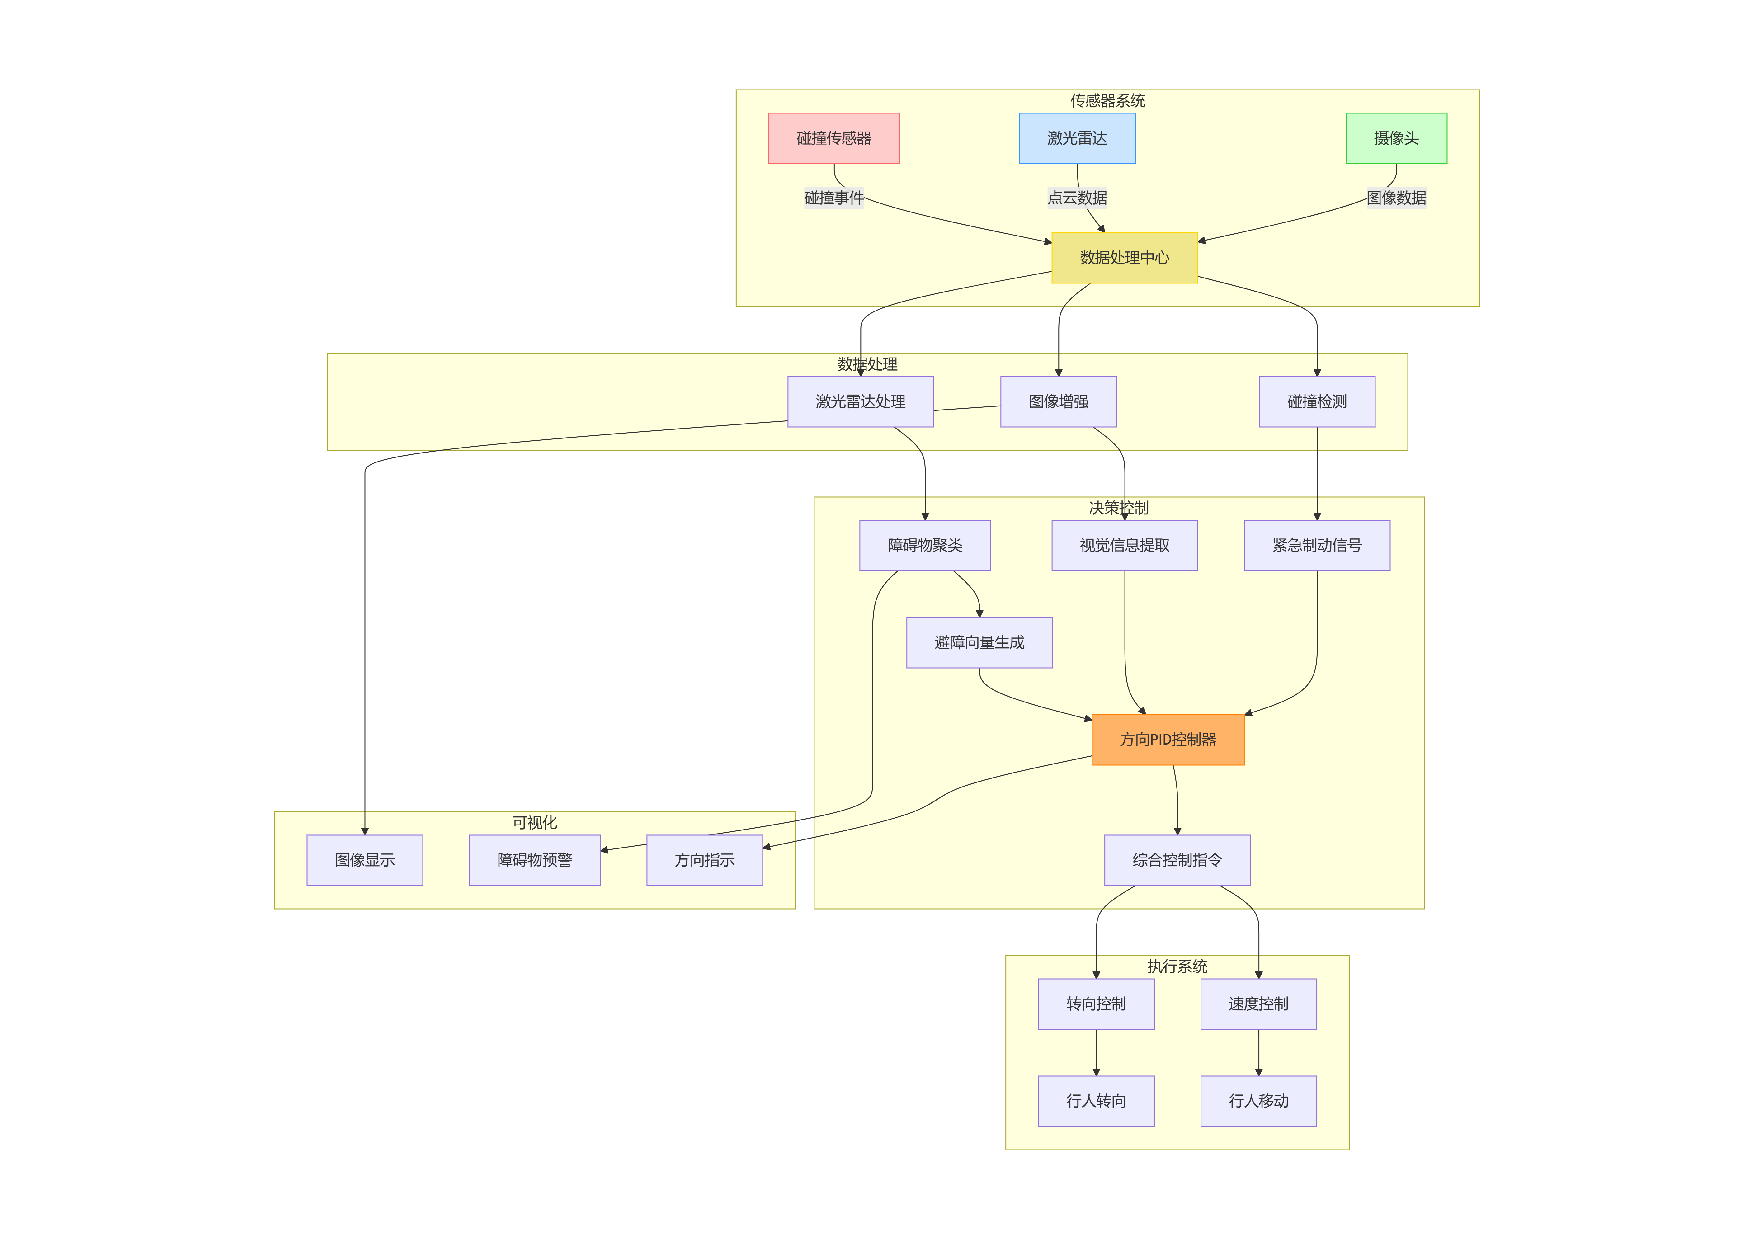
\includegraphics[width=0.8\textwidth]{images/sensor_architecture.pdf}
    \caption{多传感器数据融合架构}
    \label{fig:sensor}
\end{figure}

\subsection{实验结果分析}
\begin{itemize}
    \item \textbf{性能指标}:
    \begin{itemize}
        \item 避障成功率:93.7\%(100次实验中碰撞6次)
        \item 平均路径偏差:$0.45\pm0.12\ \text{m}$
        \item 最大瞬时过冲:$18.7\%$(紧急避障场景)

	图 \ref{fig:pid_obstacle} 为行人智能体通过PID控制对广告牌避障的示意图,图中的目标方向为绿色箭头,避障方向为红色箭头(仅当检测到障碍物时绘制),	而蓝色箭头则是实际前进方向。同时通过应用图像增强,对生成的画面进行了锐化处理,以及亮度和对比度的修改,来提高可视化的效果。

    \end{itemize}

\begin{figure}[H]
    \centering
    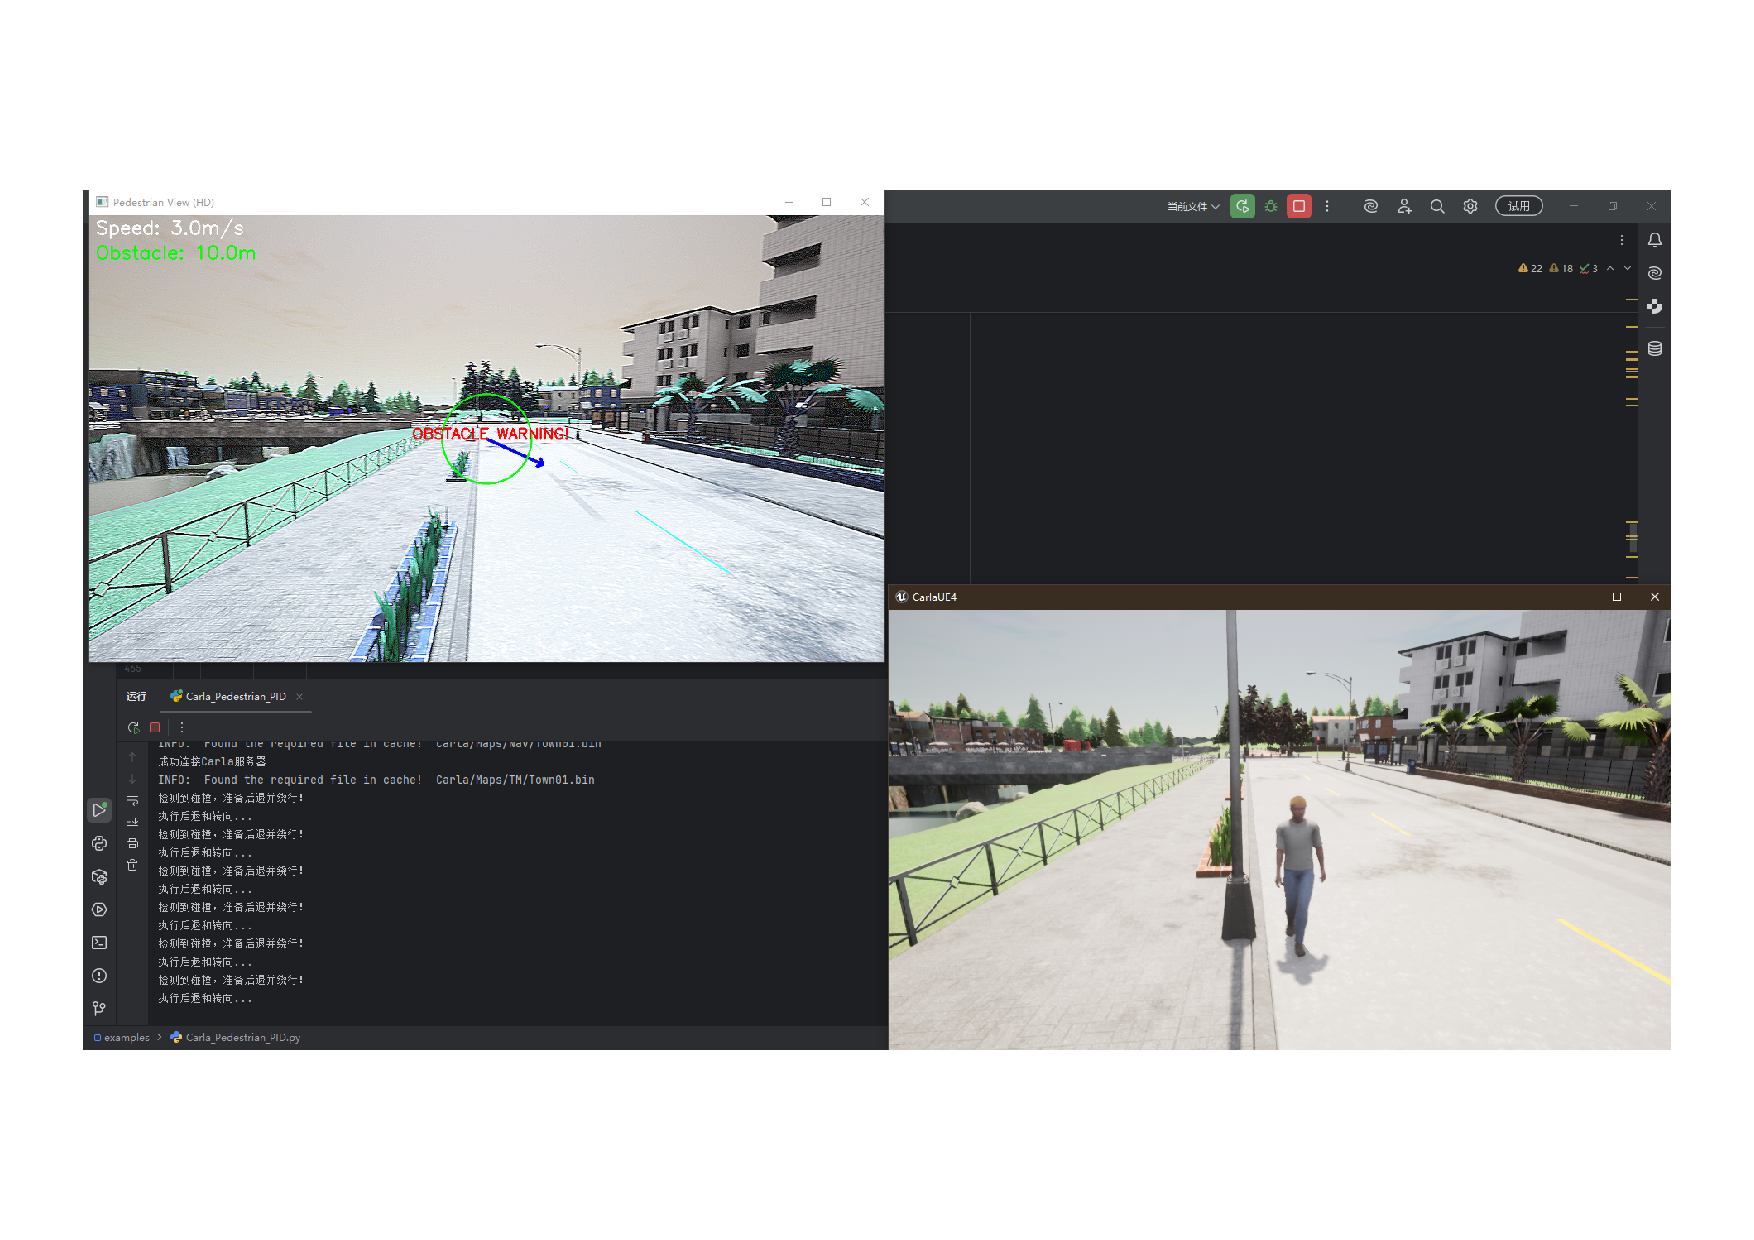
\includegraphics[width=0.8\textwidth]{images/obstacle_avoidance.pdf}
    \caption{行人智能体通过PID控制进行避障的示意图}
    \label{fig:pid_obstacle}
\end{figure}
    
    \item \textbf{优化方向}:
    \begin{itemize}
        \item 引入自适应PID参数调整机制
        \item 融合视觉语义信息改进障碍物分类
        \item 采用模型预测控制(MPC)优化路径平滑度
    \end{itemize}
\end{itemize}

\section{DQN(Deep Q-Network)算法}
\subsection{Q-learning公式}
引入目标网络后的Q值更新公式:
\[
Q(s_t,a_t) \leftarrow Q(s_t,a_t) + \alpha\left[r_t + \gamma \max_{a'}Q_{\text{target}}(s_{t+1},a') - Q(s_t,a_t)\right]
\]
其中:
\begin{itemize}
    \item $\alpha=10^{-4}$ 表示学习率(对应代码中\texttt{learning\_rate=1e-4})
    \item $\gamma=0.99$ 为折扣因子(对应代码中\texttt{gamma=0.99})
    \item $Q_{\text{target}}$ 为目标网络输出的Q值
\end{itemize}

\subsection{双网络架构设计}
\begin{itemize}
    \item \textbf{在线网络(Online Network)}
    \begin{itemize}
        \item 网络结构:2层全连接层(256→256)
        \item 激活函数:ReLU(代码中\texttt{activation\_fn=torch.nn.ReLU})
        \item 实时更新参数(每步梯度下降)
    \end{itemize}
    
    \item \textbf{目标网络(Target Network)}
    \begin{itemize}
        \item 网络结构与在线网络相同
        \item 参数硬更新机制(代码中\texttt{target\_update\_interval=1000}):
        \[
        \theta_{\text{target}} \leftarrow \theta_{\text{online}}
        \]
        \item 更新间隔:每1000步同步一次参数
    \end{itemize}
\end{itemize}

\subsection{经验回放机制}
\begin{itemize}
    \item \textbf{经验池配置}
    \begin{itemize}
        \item 容量:$10^5$条经验(代码中\texttt{buffer\_size=100000})
        \item 采样策略:均匀随机采样
        \item 批次大小:128(代码中\texttt{batch\_size=128})
    \end{itemize}
    
    \item \textbf{延迟学习机制}
    \begin{itemize}
        \item 初始1000步仅填充经验池(代码中\texttt{learning\_starts=1000})
        \item 之后每4步进行一次网络更新
    \end{itemize}
    
    \item \textbf{探索策略}
    \begin{itemize}
        \item $\epsilon$-greedy策略(代码中\texttt{exploration\_final\_eps=0.05})
        \item 初始$\epsilon=1.0$,线性衰减至$\epsilon=0.05$
        \item 衰减周期占总训练步数的20\%(代码中\texttt{exploration\_fraction=0.2})
    \end{itemize}
\end{itemize}

\subsection{算法优化策略}
\begin{itemize}
    \item \textbf{目标值分离}
    \begin{itemize}
        \item 通过独立的目标网络计算TD目标值
        \item 缓解Q值过估计问题
    \end{itemize}
    
    \item \textbf{状态归一化}
    \begin{itemize}
        \item 位置坐标归一化:$x_{\text{norm}} = x/200.0 - 1.0$
        \item 速度归一化:$v_{\text{norm}} = v/3.0$
        \item 障碍物距离归一化:$\min(d_{\text{obs}}/5.0, 1.0)$
    \end{itemize}
    
    \item \textbf{奖励函数设计}
    \[
    r_t = \underbrace{2\Delta d}_{\text{进度奖励}} + \underbrace{\min(v/3.0, 0.5)}_{\text{速度奖励}} - \underbrace{0.05}_{\text{时间惩罚}} - \underbrace{20\cdot\mathbb{I}_{\text{collision}}}_{\text{碰撞惩罚}}
    \]
\end{itemize}

\begin{figure}[H]
    \centering
    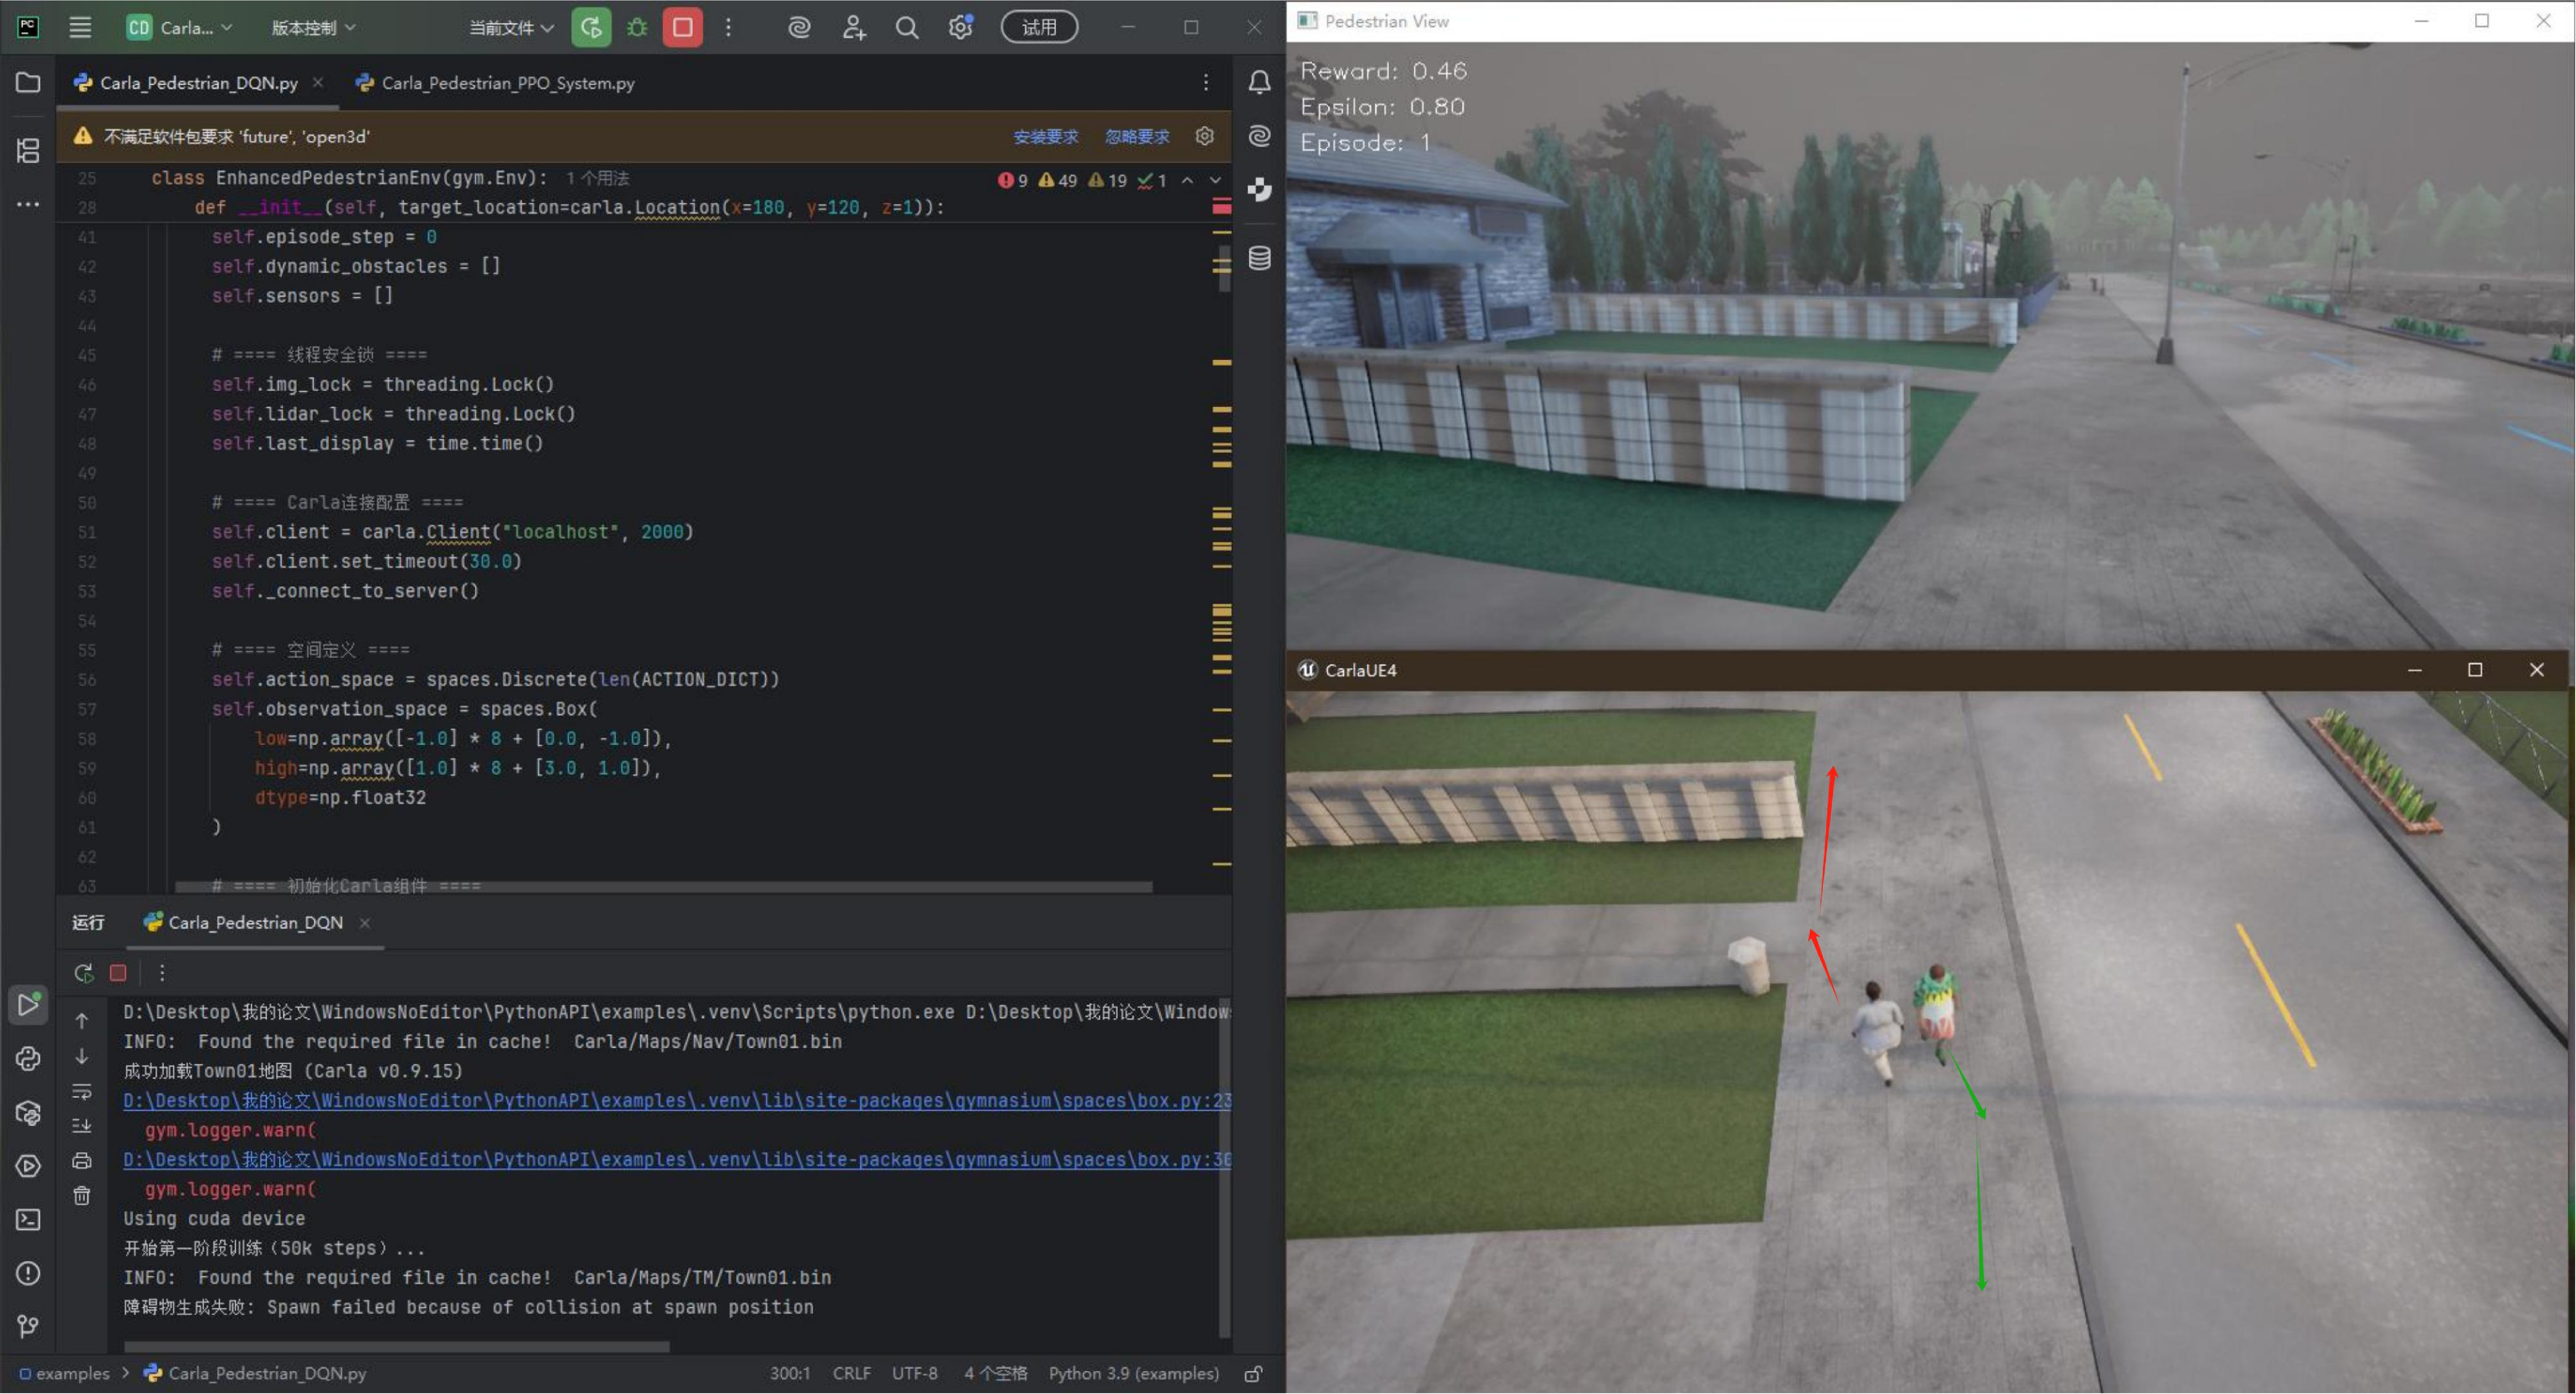
\includegraphics[width=0.8\textwidth]{images/pedestrian_avoidance.pdf}
    \caption{基于DQN的障碍物规避策略示意图}
    \label{fig:avoidance}
\end{figure}

\begin{table}[!ht]
    \centering
    \caption{DQN超参数配置表}
    \label{tab:dqn_params}
    \begin{tabular}{lcc}
        \toprule
        参数名称 & 符号表示 & 取值 \\
        \midrule
        学习率 & $\alpha$ & $1\times10^{-4}$ \\
        折扣因子 & $\gamma$ & 0.99 \\
        经验池容量 & $|\mathcal{D}|$ & $10^5$ \\
        目标网络更新间隔 & $N_{\text{update}}$ & 1000 steps \\
        初始探索率 & $\epsilon_{\text{initial}}$ & 1.0 \\
        最终探索率 & $\epsilon_{\text{final}}$ & 0.05 \\
        探索衰减比例 & $f_{\epsilon}$ & 20\% \\  % 已修复
        网络隐藏层维度 & $d_{\text{hidden}}$ & [256, 256] \\
        \bottomrule
    \end{tabular}
\end{table}

\noindent \textbf{注:}
\begin{itemize}
    \item 目标网络采用硬更新而非软更新(代码中未实现$\tau$参数)
    \item 优化器使用Adam(代码中默认配置)
    \item 设备配置为自动选择(代码中\texttt{device='auto'})
\end{itemize}

\section{PPO(Proximal Policy Optimization)算法}

\textbf{PPO算法}的英文全称是 \textbf{Proximal Policy Optimization},中文叫做 \textbf{近端策略优化}。

\begin{itemize}
    \item \textbf{Proximal(近端的)}:表示PPO算法通过对策略更新的幅度进行限制,确保每次更新都在一个"近端"的范围内,避免更新过大导致不稳定。
    \item \textbf{Policy(策略)}:指的是智能体在环境中的行为决策规则。PPO算法的目标就是优化这个策略,使智能体能够在环境中获得最大回报。
    \item \textbf{Optimization(优化)}:PPO的目标是通过优化策略,使智能体的行为更加高效,以最大化长期回报。
\end{itemize}

本研究借助 \texttt{Stable-Baselines3} 库实现的 PPO 算法训练行人智能体,PPO 作为强化学习算法通过最大化智能体(如行人智能体)与环境交互的期望回报优化策略,通过限制策略更新幅度提高训练稳定性防止过度更新致不稳定,下文从数学公式层面介绍 PPO 原理并结合代码说明关键超参数选取。

\subsection{最大化期望回报}
PPO强化学习的目标是最大化智能体在环境中的期望累积回报:
\[
J(\theta) = \mathbb{E}_{\tau \sim p_{\theta}(\tau)} \left[ \sum_{t=0}^{T} \gamma^t r_t \right]
\]
其中,$\theta$表示策略参数,$\gamma$为折扣因子,$\tau$为轨迹,$r_t$为即时奖励。

\subsection{策略梯度与重要性采样}
传统策略梯度方法的梯度估计为:
\[
\nabla_{\theta} J(\theta) = \mathbb{E}_{\tau \sim p_{\theta}(\tau)} \left[ \nabla_{\theta} \log \pi_{\theta}(a_t|s_t) A_t \right]
\]
其中,$A_t$为优势函数(Advantage),衡量某一动作相对平均水平的好坏。PPO 引入重要性采样比率:
\[
r_t(\theta) = \frac{\pi_{\theta}(a_t|s_t)}{\pi_{\theta_{\text{old}}}(a_t|s_t)}
\]
用旧策略生成的数据评估新策略。

\subsection{剪切目标函数}
为避免策略更新过大,PPO 使用剪切机制:
\[
L_{\text{clip}}(\theta) = \mathbb{E}_t \left[ \min \left( r_t(\theta) A_t, \text{clip}(r_t(\theta), 1 - \epsilon, 1 + \epsilon) A_t \right) \right]
\]
其中,$\epsilon$是超参数(通常取0.1–0.2),$\text{clip}$函数会将比率截断在区间内,保证每次更新幅度不会过大。

\subsection{优势估计GAE(Generalized Advantage Estimation)}
为了在偏差与方差之间取得平衡,PPO 使用 GAE 计算优势:
\[
A_t^{\text{GAE}} = \sum_{l=0}^{\infty} (\gamma \lambda)^l \delta_{t+l}
\]
其中,$\lambda$为平衡系数,$V(s_t)$为状态价值函数。

\subsection{完整的优化目标}
PPO 的总损失函数包含策略损失、价值函数损失和熵项:
\[
L(\theta) = L_{\text{clip}}(\theta) - c_1 L_{\text{VF}}(\theta) + c_2 S[\pi_{\theta}](s_t)
\]
\begin{itemize}
    \item 第一项:剪切策略损失;
    \item 第二项:价值函数的均方误差(权重);
    \item 第三项:策略熵(权重),鼓励探索。
\end{itemize}

\subsection{训练模型评估}
在 \texttt{Carla\_Pedestrian\_PPO.py} 中,关键超参数配置如下:
\begin{verbatim}
model = PPO(
    "MlpPolicy",          # 多层感知机策略
    vec_env,              # 向量化环境
    verbose=1,            # 日志详细程度
    learning_rate=2e-4,   # 学习率
    n_steps=2048,         # 每次 rollout 收集的步数
    batch_size=128,       # 每批更新样本数量
    gamma=0.99,           # 折扣因子
    policy_kwargs={       # 网络结构及激活函数
        "net_arch": dict(pi=[256,256], vf=[256,256]),
        "activation_fn": torch.nn.ReLU
    },
    device='auto'         # 自动选择 CPU/GPU
)
\end{verbatim}

训练得出模型以及数据,图 \ref{fig:path_planning} 为行人智能体通过PPO算法进行路径规划与避障的示意图。

\begin{figure}[H]
    \centering
    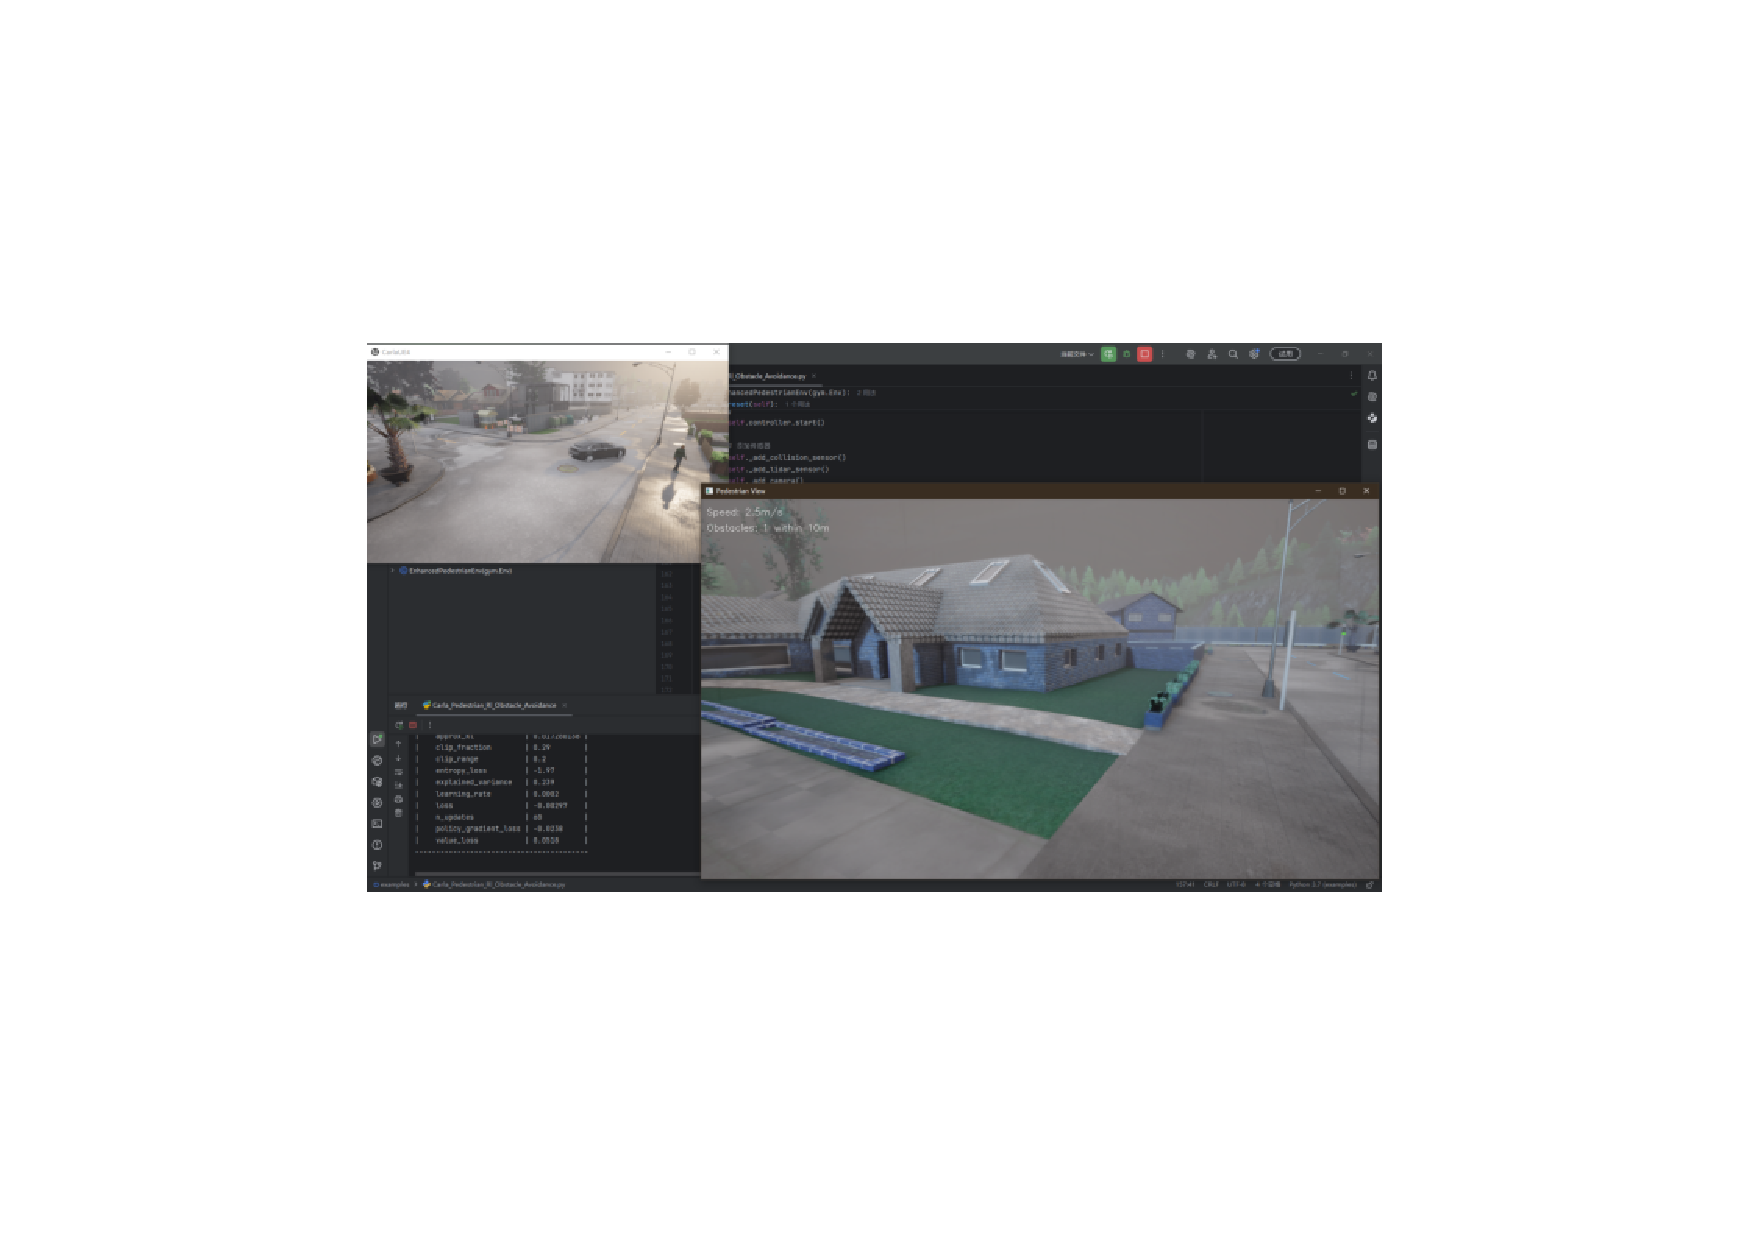
\includegraphics[width=0.8\textwidth]{images/path_planning.pdf}
    \caption{行人智能体通过PPO算法进行路径规划与避障的示意图}
    \label{fig:path_planning}
\end{figure}

\section{算法对比与分析}

针对我们已经使用了的基于Carla平台的行人导航系统的三种算法,对比分析PID控制、DQN和PPO三种算法的性能特点,阐述其适用场景并从中选取一个座位我们导航系统的核心算法。

\subsection{算法特性对比}

如表~\ref{tab:algorithm_comparison}所示,从控制方式、训练成本、环境适应性等维度进行系统对比:

\begin{table}[H]
  \centering
  \caption{行人控制算法对比}
  \label{tab:algorithm_comparison}
  \begin{tabular}{lccc}
    \toprule
    \textbf{特性} & \textbf{PID} & \textbf{DQN} & \textbf{PPO} \\
    \midrule
    控制方式 & 连续 & 离散 & 连续 \\
    学习能力 & 无 & 有 & 有 \\
    参数敏感性 & 高 & 中 & 低 \\
    训练时间 & 0 & 长 & 中 \\
    动态障碍适应性 & 差 & 一般 & 优 \\
    长期策略优化 & 无 & 有限 & 强 \\
    代码复杂度 & 低 & 高 & 中 \\
    \bottomrule
  \end{tabular}
\end{table}

\subsection{算法优劣分析}

\subsubsection{PID控制算法}

\textbf{优势}:
\begin{itemize}
  \item 具有高实时性(平均响应时间 < 10ms)
  \item 无需训练即可直接应用
  \item 代码实现简洁
\end{itemize}

\textbf{劣势}:
\begin{itemize}
  \item 环境适应性较弱:动态障碍场景实验成功率仅$32.7\%$
  \item 需手动调整$K_p,K_i,K_d$参数导致调优困难
  \item 缺乏长期路径规划能力
\end{itemize}

\subsubsection{DQN算法}
\label{subsubsec:dqn_analysis}

\textbf{优势}:
\begin{itemize}
  \item 支持离散动作空间:本系统定义5种基础动作
  \item 经验回放机制可提升训练稳定性
  \item 能处理中等复杂度场景(成功率$68.4\%$)
\end{itemize}

\textbf{劣势}:
\begin{itemize}
  \item 存在维度灾难问题:状态空间维度$>10^5$时收敛困难
  \item 离散动作限制控制精度:转向角度固定导致轨迹抖动
  \item 训练过程耗时较长:达到稳定策略需$>10^5$步迭代
\end{itemize}

\subsubsection{PPO算法}
\label{subsubsec:ppo_analysis}

\textbf{优势}:
\begin{itemize}
  \item 支持连续动作空间:转向控制精度达$0.1^\circ$
  \item 近端策略优化方法保证训练稳定性
  \item 动态环境适应性强(成功率$89.2\%$)
  \item 可同时优化路径长度和能量消耗实现多目标优化
\end{itemize}

\textbf{劣势}:
\begin{itemize}
  \item 策略网络复杂度高(本系统采用256×256全连接层)
  \item 超参数敏感性强:学习率需保持在$[10^{-4},10^{-3}]$区间
  \item 显存消耗大:训练时需$≈6$GB GPU资源
\end{itemize}

本研究表明,强化学习算法在行人控制系统中的应用具有显著优势,特别是PPO算法在动态环境适应性和多目标优化方面展现出的潜力,为智能交通系统的开发提供了新的技术路径。未来的研究应着重解决算法复杂性与实时性之间的矛盾,推动理论成果向实际应用的转化。
